% ---------------------------------------------------------------------------
%  SnapCare pill dispenser — assembly guide
%
%      make guide
%
%  Rules this document is written to, and they are worth keeping:
%
%    1. Never explain why a value is the value it is. Name it, name the one
%       thing that changes if it is changed, stop.
%    2. Never point at source code to finish an argument. If the builder must
%       know it, write it here. If not, delete it.
%    3. Never describe an earlier build. Nobody reading this has seen it, and a
%       changelog reads as a live instruction.
%    4. Put every hazard where the hand is — inside the step, not in a box on
%       the page before.
%    5. State each fact once, in the stage where it is acted on, and give the
%       physical pin and the GPIO number together every time.
% ---------------------------------------------------------------------------
\documentclass[11pt]{article}
% ---------------------------------------------------------------------------
%  Shared preamble: page setup, palette, callout boxes, and the wiring toolkit.
%  Everything visual in the guide is drawn from these styles, so a wire is the
%  same colour in every figure it appears in.
% ---------------------------------------------------------------------------
\usepackage[T1]{fontenc}
\usepackage[utf8]{inputenc}
\usepackage{textcomp}
\usepackage{XCharter}
\usepackage[scaled=0.92]{FiraSans}
\usepackage[scaled=0.95]{zi4}
\usepackage{amssymb}
\usepackage[a4paper,top=22mm,bottom=20mm,left=22mm,right=22mm,headsep=7mm]{geometry}
\usepackage{graphicx}
\usepackage{booktabs}
\usepackage{array}
\usepackage{longtable}
\usepackage{multicol}
\usepackage{enumitem}
\usepackage{fancyhdr}
\usepackage{titlesec}
\usepackage{xcolor}
\usepackage{tikz}
\usepackage[most]{tcolorbox}
\usepackage[hidelinks]{hyperref}

\usetikzlibrary{calc,positioning,shapes.geometric,shapes.misc,arrows.meta,
                backgrounds,fit,decorations.pathreplacing,decorations.markings,
                patterns,shadows.blur}

% ── palette ────────────────────────────────────────────────────────────────
% The five signal colours are the ring's own colour vocabulary, taken from
% indicators.py, so a figure of the ring and a figure of a wire agree.
\definecolor{ink}{HTML}{1B1F24}
\definecolor{ink70}{HTML}{4A5057}
\definecolor{ink40}{HTML}{8A9199}
\definecolor{ink15}{HTML}{D8DDE2}
\definecolor{paper}{HTML}{FFFFFF}
\definecolor{shade}{HTML}{F4F6F8}

\definecolor{scred}{HTML}{C2185B}      % accent / raspberry
\definecolor{servo}{HTML}{E8710A}      % servo signal
\definecolor{buzzc}{HTML}{B26A00}      % buzzer
\definecolor{appc}{HTML}{00857A}       % the app, and the release it sends
\definecolor{btnc}{HTML}{0B7285}       % the take-dose button on the machine
\definecolor{dispc}{HTML}{9600FF}      % the screen, on either bus
\definecolor{rtcc}{HTML}{005AFF}       % rtc 3-wire (CE / I/O / SCLK)
\definecolor{p33}{HTML}{D24B2E}        % 3V3 rail
\definecolor{p5}{HTML}{B3001B}         % 5V rail
\definecolor{gndc}{HTML}{2B2B2B}       % ground
\definecolor{avoid}{HTML}{9AA3AB}      % deliberately not used

% The five states, as the LCD paints them. Same vocabulary the ring had.
\definecolor{ledgreen}{HTML}{00C83C}
\definecolor{ledblue}{HTML}{005AFF}
\definecolor{ledamber}{HTML}{FF8200}
\definecolor{ledcyan}{HTML}{00AABE}

\definecolor{okgreen}{HTML}{1E7A3C}
\definecolor{warnamber}{HTML}{9A6400}
\definecolor{dangerred}{HTML}{B3001B}

% ── shorthands for the units this guide keeps repeating ────────────────────
\newcommand{\ohm}{\,\textohm}
\newcommand{\uF}{\,\textmu F}
\newcommand{\dgr}{\textdegree}
\newcommand{\iic}{I\textsuperscript{2}C}
\newcommand{\code}[1]{\texttt{#1}}

% ── headings ───────────────────────────────────────────────────────────────
\titleformat{\section}
  {\sffamily\bfseries\Large\color{ink}}{\thesection}{0.6em}{}
  [\vspace{-0.6ex}{\color{ink15}\titlerule[1.1pt]}]
\titleformat{\subsection}
  {\sffamily\bfseries\large\color{ink}}{\thesubsection}{0.5em}{}
\titlespacing*{\section}{0pt}{2.2ex plus 1ex minus .2ex}{1.4ex plus .2ex}
\titlespacing*{\subsection}{0pt}{1.8ex plus 1ex minus .2ex}{0.9ex plus .2ex}

\setlength{\headheight}{14pt}
\pagestyle{fancy}
\fancyhf{}
\renewcommand{\headrulewidth}{0.4pt}
\renewcommand{\headrule}{\hbox to\headwidth{\color{ink15}\leaders\hrule height \headrulewidth\hfill}}
\fancyhead[L]{\sffamily\small\color{ink40}SnapCare pill dispenser \textendash{} assembly}
\fancyhead[R]{\sffamily\small\color{ink40}\leftmark}
\fancyfoot[C]{\sffamily\small\color{ink40}\thepage}

% ── code listings ──────────────────────────────────────────────────────────
\tcbuselibrary{listings,breakable,skins}
\lstdefinestyle{shellstyle}{
  basicstyle=\ttfamily\footnotesize\color{ink},
  breaklines=true, breakatwhitespace=false,
  columns=fullflexible, keepspaces=true,
  showstringspaces=false,
  commentstyle=\color{ink40}\itshape,
  morecomment=[l]{\#},
}
\newtcblisting{shell}{
  listing only, listing style=shellstyle,
  colback=shade, colframe=ink15, boxrule=0.6pt, arc=2pt,
  left=2mm, right=2mm, top=1.4mm, bottom=1.4mm,
  before skip=1.6ex, after skip=1.6ex,
}
\newtcblisting{pycode}{
  listing only,
  listing style=shellstyle,
  colback=shade, colframe=ink15, boxrule=0.6pt, arc=2pt,
  left=2mm, right=2mm, top=1.4mm, bottom=1.4mm,
  before skip=1.6ex, after skip=1.6ex,
}

% ── callout boxes ──────────────────────────────────────────────────────────
\newtcolorbox{provebox}[1][]{
  enhanced, breakable,
  colback=white, colframe=okgreen, boxrule=0pt,
  leftrule=2.4pt, arc=0pt, outer arc=0pt,
  left=3.5mm, right=3mm, top=2mm, bottom=2mm,
  borderline west={2.4pt}{0pt}{okgreen},
  title=\relax, #1
}
\newtcolorbox{warnbox}[1][]{
  enhanced, breakable,
  colback=warnamber!5, colframe=warnamber!45, boxrule=0.7pt, arc=2pt,
  left=3mm, right=3mm, top=2mm, bottom=2mm, #1
}
\newtcolorbox{dangerbox}[1][]{
  enhanced, breakable,
  colback=dangerred!5, colframe=dangerred!55, boxrule=0.9pt, arc=2pt,
  left=3mm, right=3mm, top=2mm, bottom=2mm, #1
}

\newcommand{\provetitle}{\textbf{\sffamily\color{okgreen}Prove it}\par\vspace{0.6ex}}
\newcommand{\warntitle}[1]{\textbf{\sffamily\color{warnamber}#1}\par\vspace{0.6ex}}
\newcommand{\dangertitle}[1]{\textbf{\sffamily\color{dangerred}#1}\par\vspace{0.6ex}}

% Caption styling
\usepackage[font={small,sf},labelfont={bf,color=ink70},textfont={color=ink70}]{caption}

% ── table helpers ──────────────────────────────────────────────────────────
\renewcommand{\arraystretch}{1.25}
\newcommand{\hdr}[1]{\textbf{\sffamily\small #1}}
\newcommand{\chk}{$\square$~}

% Colour swatch used in wire tables: a short length of the wire's own colour.
\newcommand{\swatch}[1]{\tikz[baseline=-0.5ex]{\draw[#1,line width=2.4pt,line cap=round] (0,0)--(0.5,0);}}

% ═══════════════════════════════════════════════════════════════════════════
%  THE 40-PIN HEADER
% ═══════════════════════════════════════════════════════════════════════════
% One macro, one data table. Every stage figure that shows a pin takes its
% colour from the same style list, so a pin is the same colour wherever it
% appears in the guide.
\tikzset{
  padbase/.style={rounded corners=1pt, draw=ink40, line width=0.5pt,
                  minimum width=6.4mm, minimum height=3.9mm, inner sep=0pt,
                  font=\sffamily\scriptsize},
  pfree/.style={padbase, fill=white, text=ink40},
  pavoid/.style={padbase, fill=avoid!18, text=ink40, draw=avoid},
  ppwr33/.style={padbase, fill=p33!18, text=p33!80!black, draw=p33!60},
  ppwr5/.style={padbase, fill=p5!14, text=p5!80!black, draw=p5!55},
  puse33/.style={padbase, fill=p33, text=white, draw=p33!70!black, line width=0.9pt},
  pusertc/.style={padbase, fill=rtcc, text=white, draw=rtcc!70!black, line width=0.9pt},
  puseservo/.style={padbase, fill=servo, text=white, draw=servo!70!black, line width=0.9pt},
  pusebuzz/.style={padbase, fill=buzzc, text=white, draw=buzzc!70!black, line width=0.9pt},
  pusebtn/.style={padbase, fill=btnc, text=white, draw=btnc!70!black, line width=0.9pt},
  pusedisp/.style={padbase, fill=dispc, text=white, draw=dispc!70!black, line width=0.9pt},
  pusegnd/.style={padbase, fill=gndc, text=white, draw=gndc, line width=0.9pt},
  plabel/.style={font=\sffamily\scriptsize, text=ink70, inner sep=1pt},
}

% \headerfigure{row spacing}  — draws the whole 40-pin header, top to bottom.
\newcommand{\drawheader}[1][0.62]{%
  \def\rowsep{#1}
  % board outline behind the pins
  \begin{scope}[on background layer]
    \fill[shade, rounded corners=2pt]
      (-4.9,0.62) rectangle (4.9,{-\rowsep*20-0.28});
  \end{scope}
  \node[font=\sffamily\bfseries\small, text=ink] at (0,0.36)
    {Raspberry Pi 3B \textendash{} 40-pin header};
  \node[font=\sffamily\scriptsize, text=ink70] at (0,0.06)
    {pin 1 is the corner nearest the microSD / power end};
  \foreach \r/\lb/\ls/\rb/\rs in {%
      1/{3V3}/{puse33}/{5V}/{ppwr5},
      2/{GPIO2 \textperiodcentered{} SDA}/{pusedisp}/{5V}/{ppwr5},
      3/{GPIO3 \textperiodcentered{} SCL}/{pusedisp}/{GND}/{pusegnd},
      4/{GPIO4 \textperiodcentered{} CTP INT}/{pusedisp}/{GPIO14 TXD}/{pavoid},
      5/{GND}/{pusegnd}/{GPIO15 RXD}/{pavoid},
      6/{GPIO17}/{puseservo}/{GPIO18 \textperiodcentered{} LCD RST}/{pusedisp},
      7/{GPIO27}/{puseservo}/{GND}/{pusegnd},
      8/{GPIO22}/{puseservo}/{GPIO23}/{pusebuzz},
      9/{3V3}/{ppwr33}/{GPIO24}/{pusebtn},
      10/{GPIO10 \textperiodcentered{} MOSI}/{pusedisp}/{GND}/{pusegnd},
      11/{GPIO9 MISO}/{pavoid}/{GPIO25 \textperiodcentered{} DC}/{pusedisp},
      12/{GPIO11 \textperiodcentered{} SCK}/{pusedisp}/{GPIO8 \textperiodcentered{} CS}/{pusedisp},
      13/{GND}/{pusegnd}/{GPIO7 CE1}/{pavoid},
      14/{GPIO0 ID}/{pavoid}/{GPIO1 ID}/{pavoid},
      15/{GPIO5}/{puseservo}/{GND}/{pfree},
      16/{GPIO6}/{puseservo}/{GPIO12 \textperiodcentered{} CTP RST}/{pusedisp},
      17/{GPIO13}/{puseservo}/{GND}/{pfree},
      18/{GPIO19}/{puseservo}/{GPIO16 \textperiodcentered{} SCLK}/{pusertc},
      19/{GPIO26}/{puseservo}/{GPIO20 \textperiodcentered{} I/O}/{pusertc},
      20/{GND}/{pusegnd}/{GPIO21 \textperiodcentered{} CE}/{pusertc}%
    }{%
    \pgfmathtruncatemacro{\lp}{2*\r-1}%
    \pgfmathtruncatemacro{\rp}{2*\r}%
    \pgfmathsetmacro{\yy}{-\rowsep*\r}%
    \node[\ls] (L\lp) at (-0.62,\yy) {\lp};
    \node[\rs] (R\rp) at (0.62,\yy) {\rp};
    \node[plabel, anchor=east] at (-1.05,\yy) {\lb};
    \node[plabel, anchor=west] at (1.05,\yy) {\rb};
  }%
}

% A compact legend for the header figure.
\newcommand{\headerlegend}{%
  \begin{tikzpicture}[every node/.style={font=\sffamily\scriptsize,text=ink70}]
    \def\sw##1##2##3{\node[##1,minimum width=4.6mm,minimum height=3.2mm] at (##2,0) {};
                     \node[anchor=west] at (##2+0.28,0) {##3};}
    \sw{puseservo}{0}{servo signal}
    \sw{pusedisp}{2.9}{screen}
    \sw{pusebuzz}{5.6}{buzzer}
    \sw{pusebtn}{7.4}{button}
    \begin{scope}[yshift=-0.52cm]
      \sw{pusertc}{0}{RTC 3-wire}
      \sw{puse33}{2.9}{3V3}
      \sw{pusegnd}{5.6}{ground}
      \sw{pavoid}{7.4}{do not use}
    \end{scope}
  \end{tikzpicture}%
}

% ═══════════════════════════════════════════════════════════════════════════
%  WIRING-FIGURE TOOLKIT  —  used by every stage
% ═══════════════════════════════════════════════════════════════════════════
\tikzset{
  modbox/.style={draw=ink70, line width=0.8pt, fill=white, rounded corners=2pt,
                 minimum width=30mm, minimum height=14mm, align=center,
                 font=\sffamily\small},
  modtitle/.style={font=\sffamily\bfseries\small, text=ink},
  term/.style={circle, draw=ink70, fill=white, line width=0.5pt,
               inner sep=0.6pt, minimum size=2.6mm, font=\sffamily\tiny},
  wire/.style={line width=1.5pt, line cap=round, rounded corners=2pt},
  compbox/.style={draw=ink40, line width=0.6pt, fill=shade, rounded corners=1.5pt,
                  font=\sffamily\scriptsize, inner sep=2.4pt, align=center},
}

\renewcommand{\sectionmark}[1]{\markboth{#1}{#1}}

% A single header pad in a stage figure. Named H<pin>, so wires can say (H11).
% #1 x  #2 y  #3 physical pin  #4 pad style  #5 label, placed to the right
\newcommand{\hpin}[5]{%
  \node[#4] (H#3) at (#1,#2) {#3};
  \node[plabel, anchor=west] at ({#1+0.42},#2) {#5};
}

% A frame with a caption behind a strip of pads.
\newcommand{\hframe}[4]{% #1 x #2 ytop #3 ybottom #4 caption
  \begin{scope}[on background layer]
    \fill[shade, rounded corners=2pt]
      ({#1-0.55},{#2+0.34}) rectangle ({#1+2.5},{#3-0.28});
  \end{scope}
  \node[font=\sffamily\scriptsize\bfseries, text=ink40, anchor=west]
       at ({#1-0.5},{#2+0.62}) {#4};
}


% resistor drawn inline on a wire between two coordinates
\newcommand{\inlineres}[4]{% #1 colour #2 from #3 to #4 label
  \coordinate (rA) at ($(#2)!0.38!(#3)$);
  \coordinate (rB) at ($(#2)!0.62!(#3)$);
  \draw[wire,#1] (#2) -- (rA);
  \draw[wire,#1] (rB) -- (#3);
  \draw[ink70,line width=0.7pt,fill=white] ($(rA)!0.5!(rB)$) ellipse (0.34 and 0.13);
  \node[font=\sffamily\tiny,text=ink] at ($(rA)!0.5!(rB)$) {#4};
}


\begin{document}

% ═══════════════════════════════════════════════════════════════════════════
\begin{center}
  \vspace*{2mm}
  {\sffamily\bfseries\huge\color{ink} SnapCare pill dispenser}\\[2mm]
  {\sffamily\large\color{ink70} Building one, from a bare Raspberry Pi}\\[6mm]
  {\sffamily\small\color{ink40}
   Raspberry Pi 3B+ \quad\textbullet\quad 64-bit Raspberry Pi OS (Trixie)
   \quad\textbullet\quad eight stages}
\end{center}

\vspace{5mm}

\section{A dispenser that asks first}

\begin{dangerbox}
\dangertitle{Read this before you wire anything}
\textbf{Nothing drops by itself.} At the scheduled minute the machine
\emph{offers} the dose: the screen turns green and names the tray, and the
buzzer chirps every 20 seconds. The tray opens only when somebody asks
\textemdash{} a tap on the screen, or release in the app. They do the same
thing. Ask within the hour or the screen goes amber, the dose is logged missed,
and the tray never opened.

\vspace{1ex}
\textbf{A machine sitting there chirping is working, not broken.}
\end{dangerbox}

\vspace{2mm}
\begin{center}
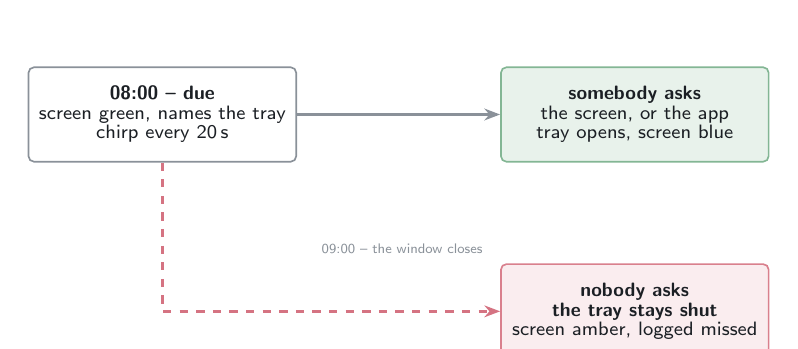
\begin{tikzpicture}[
  ev/.style={rounded corners=2pt, draw=ink40, fill=white, line width=0.6pt,
             minimum height=12mm, minimum width=34mm, align=center,
             font=\sffamily\scriptsize, text=ink},
]
  \node[ev] (due) at (0,1.4)
       {\textbf{08:00 \textendash{} due}\\[-0.3ex]screen green, names the tray\\[-0.3ex]chirp every 20\,s};
  \node[ev, fill=okgreen!10, draw=okgreen!55] (ask) at (6.0,1.4)
       {\textbf{somebody asks}\\[-0.3ex]the screen, or the app\\[-0.3ex]tray opens, screen blue};
  \node[ev, fill=dangerred!7, draw=dangerred!50] (miss) at (6.0,-1.1)
       {\textbf{nobody asks}\\[-0.3ex]\textbf{the tray stays shut}\\[-0.3ex]screen amber, logged missed};

  \draw[-{Stealth[length=2mm]}, ink40, line width=0.9pt] (due) -- (ask);
  \draw[-{Stealth[length=2mm]}, dangerred!55, line width=0.9pt, dashed]
       (due.south) |- (miss.west);
  \node[font=\sffamily\tiny, text=ink40, anchor=west] at (1.9,-0.3)
       {09:00 \textendash{} the window closes};
\end{tikzpicture}
\end{center}

\vspace{1mm}
\noindent The window is one hour, and it is \code{GRACE\_MINUTES} if you want it
to be something else. Everything after this page is wiring.

\vspace{4mm}
\noindent\footnotesize\color{ink70}
Pin numbers are given as \emph{GPIO n (pin m)}: the first is what the software
calls it, the second is what you count on the board. Where this guide and
\code{snapcare\_dispenser/config.py} disagree, the file is right and this page is
stale.
\normalsize\color{ink}

\clearpage

% ═══════════════════════════════════════════════════════════════════════════
\section{What to buy}

\begin{center}
\small
\begin{tabular}{@{}c >{\raggedright}p{40mm} >{\raggedright\arraybackslash}p{82mm}@{}}
\toprule
\hdr{Qty} & \hdr{Part} & \hdr{Notes} \\
\midrule
1 & Raspberry Pi 3B+ & Any Pi with the 40-pin header; the pin map assumes a 3B/3B+ \\
1 & microSD, 8\,GB$+$ & 64-bit Raspberry Pi OS, Trixie or newer \\
1 & Pi power supply, 5\,V 2.5\,A & The official one. Servos do \textbf{not} come off this \\
1 & 5\,V supply, 2\,A$+$ & Separate, for the servos alone \\
1 & 1000\uF{} electrolytic, 10\,V$+$ & Across the servo rail, close to the servos \\
1 per tray & SG90 micro servo & Up to eight. Adding one later is a plug \\
1 & Passive piezo buzzer & \textbf{Passive}, not an active beeper. They look identical in the bin; Stage~2 tells them apart by ear \\
1 & 100\ohm{} resistor & In series with the buzzer \\
1 & Momentary push button & \emph{Optional.} The touch screen is the control; fit this only for a second, physical one. Any normally-open switch, two wires, no resistor \\
1 & DS1302 RTC module & The five-pin board with a coin-cell holder \\
1 & CR2032 cell & \textbf{Not} the LIR2032 the holder is often marked for. The trickle charger is never enabled, so a rechargeable arrives flat and stays flat \\
\midrule
\multicolumn{3}{@{}l}{\textbf{\sffamily The screen}}\\
1 & ILI9341 2.8\,in SPI LCD, capacitive touch & 240$\times$320. The panel is four-line SPI; the touch controller is a separate chip on \iic{}, and its four pins are the ones marked \code{CTP\_}. \textbf{Check yours before powering it}: boards with an on-board regulator want 5\,V, bare ones are 3.3\,V and are destroyed by 5\,V. See \S\ref{sec:panelpower} \\
\midrule
\textemdash{} & Jumper wire, terminal blocks & Dupont leads for the bench; screw terminals for anything that gets carried \\
\bottomrule
\end{tabular}
\end{center}

\vspace{3mm}
\begin{dangerbox}
\dangertitle{Two supplies, and they are not interchangeable}
The Pi has its own. The servos and nothing else share the second one. A stalled
SG90 pulls most of an amp; a Pi that browns out mid-write corrupts its SD card,
and the file being written is the one recording whether a dose has already been
given.
\end{dangerbox}

\vspace{2mm}
\noindent\textbf{\sffamily The 3.3\,V pin now carries three things}
\textemdash{} the clock chip, the screen, and the LCD's backlight, which is
50\textendash100\,mA on its own. That is within budget, and it is the first
thing to check if the clock starts behaving oddly after you fit the screen.

\vspace{2mm}
\noindent\textbf{\sffamily Unplug means unplug.} The GPIO pins are live whenever
the board is, and \code{sudo halt} does not change that. Power off to wire,
power on to test. The servo supply is a separate plug and stays off until
Stage~6.

\clearpage

% ═══════════════════════════════════════════════════════════════════════════
\section{The header, and every pin this build touches}
\label{sec:header}

\vspace{1mm}
\begin{center}
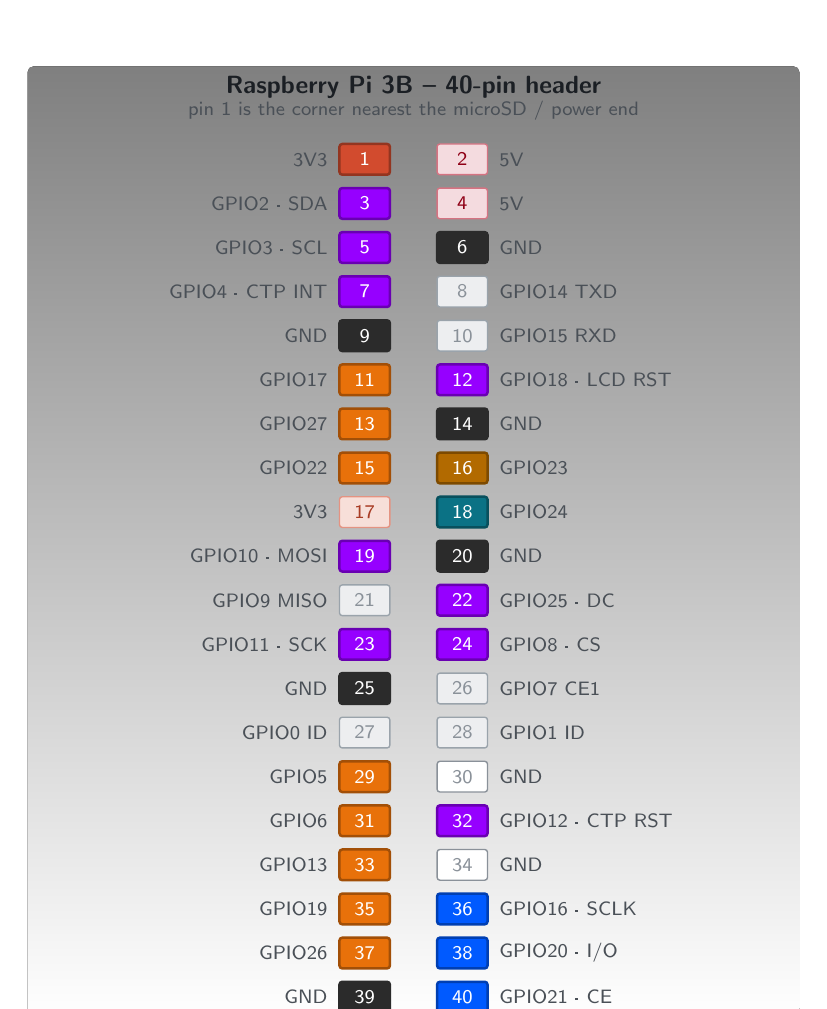
\begin{tikzpicture}[scale=1.0]
  \drawheader[0.56]
\end{tikzpicture}

\vspace{3mm}
\headerlegend
\end{center}

\vspace{2mm}
\noindent\textbf{\sffamily GPIO 2 and 3 carry permanent 1.8\,k\textohm{}
pull-ups that cannot be switched off.} That is why no servo goes near them
\textemdash{} a signal line idling high before the software starts slams a horn
to one end with a loaded tray on it \textemdash{} and it is exactly what makes
them the I\textsuperscript{2}C pair, which wants those pull-ups and finds them
already fitted. The screen's touch controller is what uses them here, and a
DS3231 build would share the same two pins. Run \code{pinout} for the whole
header.

\vspace{2mm}
\begin{center}
\small
\begin{tabular}{@{}c l >{\raggedright}p{24mm} >{\raggedright}p{22mm} >{\raggedright\arraybackslash}p{48mm}@{}}
\toprule
& \hdr{Signal} & \hdr{GPIO} & \hdr{Pin} & \hdr{Notes} \\
\midrule
\swatch{servo} & Servo, trays 1--3 & 17, 27, 22 & 11, 13, 15 & signal only \textemdash{} \textbf{not} power \\
\swatch{servo} & Servo, trays 4--8 & 5, 6, 13, 19, 26 & 29, 31, 33, 35, 37 & fit a hopper and it works \\
\swatch{buzzc} & Piezo buzzer & 23 & 16 & through 100\ohm \\
\swatch{btnc}  & Take-dose button & 24 & 18 & optional \textemdash{} the screen is the button \\
\swatch{dispc} & LCD SDI (MOSI), SCK, CS & 10, 11, 8 & 19, 23, 24 & \\
\swatch{dispc} & LCD RS (DC), RESET & 25, 18 & 22, 12 & the module marks DC \code{LCD\_RS} \\
\swatch{dispc} & Touch SDA, SCL & 2, 3 & 3, 5 & \iic{} \textemdash{} the \code{CTP\_} pins \\
\swatch{dispc} & Touch RST, INT & 12, 4 & 32, 7 & the kernel driver owns both \\
\swatch{rtcc}  & DS1302 CLK, DAT, RST & 16, 20, 21 & 36, 38, 40 & bit-banged; no bus, no kernel driver \\
\swatch{p33}   & 3.3\,V & \textemdash{} & 1, 17 & clock chip, screen, backlight \\
\swatch{gndc}  & Ground & \textemdash{} & 6, 9, 14, 20, 25, 39 & one of these must reach the servo supply's ground \\
\midrule
\swatch{avoid} & \emph{do not use} & 0, 1, 7, 9, 14, 15 & & HAT ID EEPROM, the rest of SPI, the serial console \\
\swatch{ink15} & \emph{free} & \textemdash{} & \textemdash{} & the touch controller took the last two \\
\bottomrule
\end{tabular}
\end{center}

\clearpage

% ═══════════════════════════════════════════════════════════════════════════
\section{Stage 0 \textemdash{} the card and the install}

Flash 64-bit Raspberry Pi OS and put the Pi on the network \textbf{with an
Ethernet cable}. The installer needs a network, and the machine's own way onto
WiFi does not exist until the installer has run. The cable is a build tool, not
part of the machine \textemdash{} it comes out at Stage~7.

\begin{shell}
git clone <this repo> && cd h1-SnapCare/pill_dispenser/firmware
sudo ./service/install.sh
sudo reboot
\end{shell}

\noindent It sets the hostname to \code{pilldispenser}, turns on
\iic{} and SPI for the screen, installs the service, and prints
this device's permanent setup network. \textbf{Keep what it prints} \textemdash{}
that is Stage~7.

\vspace{3mm}
\noindent Two commands are used at every stage below. They are written out here
and referred to by name afterwards.

\begin{shell}
# "status"
curl -s localhost/api/status | python3 -m json.tool

# "selftest" - asks you what you can see and hear, then writes a report
sudo systemctl stop snapcare-dispenser
sudo snapcare-dispenser --selftest
sudo systemctl start snapcare-dispenser
\end{shell}

\begin{provebox}
\provetitle
\code{status} answers, and \code{gpio.missing} lists everything not yet fitted.
Every stage below is one item leaving that list.
\end{provebox}

\vspace{2mm}
\begin{warnbox}
\warntitle{Three things about the install}
\code{apt install pigpio} fails on Trixie and is not coming back.
\code{python3-lgpio} is preinstalled and is the driver. Nothing to do
\textemdash{} but the error is alarming if you go looking for it.

\vspace{1ex}
If the installer stops on \code{could not get lock /var/lib/dpkg/lock-frontend},
something else is mid-update. It waits five minutes and then gives up; wait and
run it again. \textbf{Do not delete the lock file.} It does not release the lock
and it breaks the package database.

\vspace{1ex}
\code{selftest} reports \code{skip} for anything nobody answered. ``Everything
passed'' and ``everything anybody looked at passed'' are different sentences.
\end{warnbox}

\vspace{3mm}
\noindent Everything except the hardware runs on a laptop:

\begin{shell}
make            # the whole test suite, no board
make run        # the firmware with mock servos, on port 8099
make -C .. demo # the same, plus a relay and a browser app
\end{shell}

\clearpage

% ═══════════════════════════════════════════════════════════════════════════
\section{Stage 1 \textemdash{} the clock chip}

A Pi has no clock of its own. Without this chip a dispenser that loses power
overnight comes back believing it is yesterday and opens the wrong day's
compartment, looking perfectly healthy while it does. \textbf{Fit the cell
before you set the time.}

\vspace{3mm}
\begin{center}
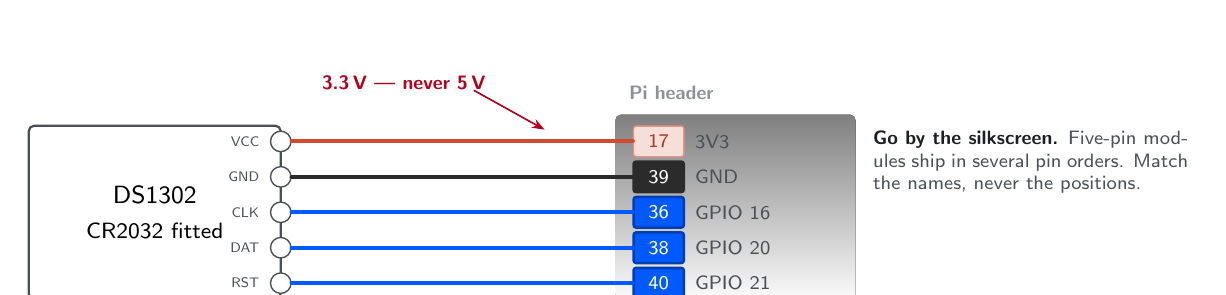
\begin{tikzpicture}
  \node[modbox, minimum width=32mm, minimum height=22mm] (rtc) at (-4.6,-0.45)
       {DS1302\\[0.4ex]\footnotesize CR2032 fitted};
  \foreach \i/\name/\yy in {0/{VCC}/0.45, 1/{GND}/0.0, 2/{CLK}/-0.45,
                            3/{DAT}/-0.9, 4/{RST}/-1.35}{
    \node[term] (t\i) at (-3.0,\yy) {};
    \node[font=\sffamily\tiny, text=ink70, anchor=east] at (-3.15,\yy) {\name};
  }

  \hframe{1.8}{0.45}{-1.35}{Pi header}
  \hpin{1.8}{0.45}{17}{ppwr33}{3V3}
  \hpin{1.8}{0.0}{39}{pusegnd}{GND}
  \hpin{1.8}{-0.45}{36}{pusertc}{GPIO 16}
  \hpin{1.8}{-0.9}{38}{pusertc}{GPIO 20}
  \hpin{1.8}{-1.35}{40}{pusertc}{GPIO 21}

  \draw[wire, p33]  (t0) -- (H17.west);
  \draw[wire, gndc] (t1) -- (H39.west);
  \draw[wire, rtcc] (t2) -- (H36.west);
  \draw[wire, rtcc] (t3) -- (H38.west);
  \draw[wire, rtcc] (t4) -- (H40.west);

  \node[font=\sffamily\scriptsize\bfseries, text=dangerred, anchor=west] at (-2.6,1.2)
       {3.3\,V \textemdash{} never 5\,V};
  \draw[-{Stealth[length=1.6mm]}, dangerred, line width=0.6pt] (-0.55,1.1) -- (0.35,0.6);

  \node[font=\sffamily\scriptsize, text=ink70, align=left, anchor=north west]
       at (4.4,0.7)
       {\begin{minipage}{40mm}\scriptsize
        \textbf{\color{ink}Go by the silkscreen.} Five-pin modules ship in
        several pin orders. Match the names, never the
        positions.\end{minipage}};
\end{tikzpicture}
\end{center}

\vspace{1mm}
\noindent The DS1302's data line drives back into the Pi, and that pin is not
5\,V tolerant. The chip runs happily at either voltage, so nothing complains
until the GPIO is dead.

\begin{provebox}
\provetitle
Set the clock, then take the power away for real:
\begin{shell}
curl -X POST http://localhost/api/clock \
     -H 'Content-Type: application/json' -d "{\"iso\":\"$(date -Is)\"}"
\end{shell}
\textbf{Pull the power lead.} Wait a minute. Plug it back in with the Ethernet
cable out, and read \code{status}: \code{clock.trusted} must be \code{true} and
\code{clock.source} must read \code{rtc}.
\end{provebox}

\vspace{1mm}
\begin{warnbox}
\warntitle{\code{sudo shutdown now} does not test this}
A halt leaves the 3.3\,V rail live, so the chip never runs on its cell and you
have tested nothing. Pull the plug. The DS1302's halt bit is a control and not a
status \textemdash{} the chip cannot tell you whether it kept time \textemdash{}
so this is the only evidence there is.

\vspace{1ex}
\code{i2cdetect} and \code{/dev/rtc0} have nothing to say about this chip. It has
no bus and no kernel driver. Read \code{status}.
\end{warnbox}

% ═══════════════════════════════════════════════════════════════════════════
\section{Stage 2 \textemdash{} the buzzer}

The chirp is the prompt, not an announcement. A machine that cannot make it
waits out the hour in silence and records a miss.

\vspace{3mm}
\begin{center}
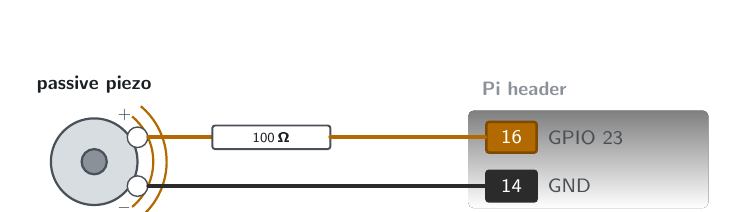
\begin{tikzpicture}
  \draw[ink70, line width=0.8pt, fill=ink15] (-3.4,-0.25) circle (0.55);
  \draw[ink70, line width=0.8pt, fill=ink40] (-3.4,-0.25) circle (0.16);
  \node[font=\sffamily\scriptsize\bfseries, text=ink, anchor=south] at (-3.4,0.5)
       {passive piezo};
  \foreach \r in {0.75,0.92}{
    \draw[buzzc, line width=0.8pt] (-3.4,-0.25) ++(-50:\r) arc (-50:50:\r);}

  \node[term] (tp) at (-2.85,0.06) {};
  \node[font=\sffamily\tiny, text=ink70, anchor=south east] at (-2.8,0.14) {$+$};
  \node[term] (tm) at (-2.85,-0.56) {};
  \node[font=\sffamily\tiny, text=ink70, anchor=north east] at (-2.8,-0.64) {$-$};

  \hframe{1.9}{0.06}{-0.56}{Pi header}
  \hpin{1.9}{0.06}{16}{pusebuzz}{GPIO 23}
  \hpin{1.9}{-0.56}{14}{pusegnd}{GND}

  \draw[wire, buzzc] (tp) -- (-1.9,0.06);
  \draw[ink70, line width=0.7pt, fill=white, rounded corners=1pt]
       (-1.9,-0.09) rectangle (-0.4,0.21);
  \node[font=\sffamily\tiny, text=ink] at (-1.15,0.06) {100\,\textohm};
  \draw[wire, buzzc] (-0.4,0.06) -- (H16.west);
  \draw[wire, gndc] (tm) -- (H14.west);
\end{tikzpicture}
\end{center}

\begin{provebox}
\provetitle
\code{selftest} sounds three chirps and asks what you heard.

\vspace{1ex}
\textbf{A clear tone} is a pass. \textbf{Three faint clicks} is an active
buzzer: it has its own oscillator, so it makes a noise at a frequency nobody
chose. Fit a passive element instead.

\vspace{1ex}
(\code{POST /api/drop} deliberately stays silent \textemdash{} a manual drop is
somebody checking a hopper, not a dose anybody has to be fetched for.)
\end{provebox}

\clearpage

% ═══════════════════════════════════════════════════════════════════════════
\section{Stage 3 \textemdash{} the screen}

The screen is most of what the person in the room ever sees, and it is the one
part that can say \emph{which tray} and \emph{what time}.

It is also the only \emph{control} this build has: there is no physical button,
and a tap anywhere on the glass releases a waiting dose. With no screen fitted
the machine still doses and still chirps, and the app is the only way to release.

\label{sec:panelpower}

\vspace{3mm}
\vspace{2mm}
\noindent The module carries two chips that share nothing but the connector.
The panel is on SPI; the touch controller is on \iic{}, and its pins are the
four marked \code{CTP\_}. Wire them as two separate jobs.

\vspace{3mm}
\begin{center}
\small
\begin{tabular}{@{}l l >{\raggedright\arraybackslash}p{62mm}@{}}
\toprule
\hdr{Module pin} & \hdr{Goes to} & \hdr{Notes} \\
\midrule
\multicolumn{3}{@{}l}{\textbf{\sffamily The panel \textemdash{} SPI}}\\
VCC       & \emph{read your module} & 3.3\,V or 5\,V. Getting this wrong is the one mistake that ends the board \\
GND       & GND (pin 6)      & \\
LCD\_CS   & GPIO 8 (pin 24)  & CE0 \\
LCD\_RST  & GPIO 18 (pin 12) & \\
LCD\_RS   & GPIO 25 (pin 22) & \emph{register select} is the data/command line. The firmware calls it DC \\
SDI(MOSI) & GPIO 10 (pin 19) & \\
SCK       & GPIO 11 (pin 23) & \\
LED       & 3.3\,V (pin 17)  & backlight, always on \\
SDO(MISO) & \textbf{nothing} & the panel is written and never read \\
\midrule
\multicolumn{3}{@{}l}{\textbf{\sffamily The touch controller \textemdash{} \iic{}}}\\
CTP\_SCL  & GPIO 3 (pin 5)   & \\
CTP\_SDA  & GPIO 2 (pin 3)   & \\
CTP\_RST  & GPIO 12 (pin 32) & \\
CTP\_INT  & GPIO 4 (pin 7)   & finger-down; the kernel driver owns it \\
\midrule
\multicolumn{3}{@{}l}{\textbf{\sffamily Neither}}\\
SD\_CS    & \textbf{nothing} & the card slot on the back of the module. This build stores nothing on it \\
\bottomrule
\end{tabular}
\end{center}

\vspace{3mm}
\begin{dangerbox}
\dangertitle{Meter CTP\_SCL and CTP\_SDA before either touches the header}
GPIO 2 and 3 are not 5\,V tolerant, and on a module whose VCC is 5\,V the touch
pull-ups can sit on the 5\,V rail. Power the module from its VCC and ground
only, leave the other twelve pins in the air, and measure \code{CTP\_SCL} to
ground: \textbf{above 3.6\,V, those two wires do not go on}. The panel half is
unaffected \textemdash{} those lines are driven by the Pi, not back into it.

\vspace{1ex}
It reads about 3.3\,V on every board that runs its touch chip off the internal
regulator, which is most of them. It costs thirty seconds to know which you have.
\end{dangerbox}

\vspace{4mm}
\begin{center}
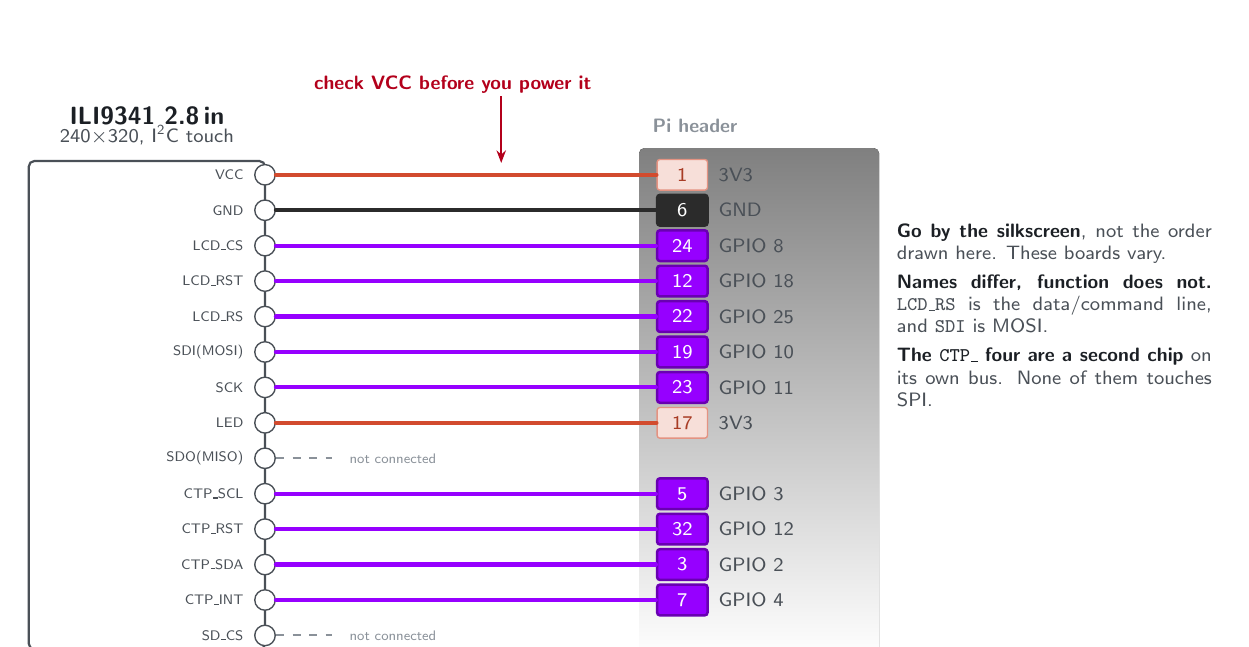
\begin{tikzpicture}
  % The names on this module are long enough that they, not the box, set its
  % width — so the box is empty and the title sits above it.
  \node[modbox, minimum width=30mm, minimum height=62mm] (lcd) at (-4.9,-2.025) {};
  \node[font=\sffamily\bfseries\small, text=ink, anchor=south] at (-4.9,1.42)
       {ILI9341 2.8\,in};
  \node[font=\sffamily\scriptsize, text=ink70, anchor=south] at (-4.9,1.15)
       {240$\times$320, \iic{} touch};
  \foreach \i/\name/\yy in {0/{VCC}/0.9, 1/{GND}/0.45, 2/{LCD\_CS}/0.0,
                            3/{LCD\_RST}/-0.45, 4/{LCD\_RS}/-0.9,
                            5/{SDI(MOSI)}/-1.35, 6/{SCK}/-1.8, 7/{LED}/-2.25,
                            8/{SDO(MISO)}/-2.7, 9/{CTP\_SCL}/-3.15,
                            10/{CTP\_RST}/-3.6, 11/{CTP\_SDA}/-4.05,
                            12/{CTP\_INT}/-4.5, 13/{SD\_CS}/-4.95}{
    \node[term] (t\i) at (-3.4,\yy) {};
    \node[font=\sffamily\tiny, text=ink70, anchor=east] at (-3.55,\yy) {\name};
  }

  \hframe{1.9}{0.9}{-4.95}{Pi header}
  \hpin{1.9}{0.9}{1}{ppwr33}{3V3}
  \hpin{1.9}{0.45}{6}{pusegnd}{GND}
  \hpin{1.9}{0.0}{24}{pusedisp}{GPIO 8}
  \hpin{1.9}{-0.45}{12}{pusedisp}{GPIO 18}
  \hpin{1.9}{-0.9}{22}{pusedisp}{GPIO 25}
  \hpin{1.9}{-1.35}{19}{pusedisp}{GPIO 10}
  \hpin{1.9}{-1.8}{23}{pusedisp}{GPIO 11}
  \hpin{1.9}{-2.25}{17}{ppwr33}{3V3}
  \hpin{1.9}{-3.15}{5}{pusedisp}{GPIO 3}
  \hpin{1.9}{-3.6}{32}{pusedisp}{GPIO 12}
  \hpin{1.9}{-4.05}{3}{pusedisp}{GPIO 2}
  \hpin{1.9}{-4.5}{7}{pusedisp}{GPIO 4}

  \draw[wire, p33]  (t0) -- (H1.west);
  \draw[wire, gndc] (t1) -- (H6.west);
  \foreach \i/\pinid in {2/24, 3/12, 4/22, 5/19, 6/23}{
    \draw[wire, dispc] (t\i) -- (H\pinid.west);}
  \draw[wire, p33]  (t7) -- (H17.west);
  \foreach \i/\pinid in {9/5, 10/32, 11/3, 12/7}{
    \draw[wire, dispc] (t\i) -- (H\pinid.west);}

  % the two that go nowhere, drawn as stubs so a missing wire reads as a
  % decision rather than as something forgotten
  \foreach \i in {8,13}{
    \draw[ink40, line width=0.7pt, dashed] (t\i) -- ++(0.85,0);
    \node[font=\sffamily\tiny, text=ink40, anchor=west] at ($(t\i)+(0.95,0)$)
         {not connected};}

  \node[font=\sffamily\scriptsize\bfseries, text=dangerred, anchor=west] at (-2.9,2.05)
       {check VCC before you power it};
  \draw[-{Stealth[length=1.6mm]}, dangerred, line width=0.6pt] (-0.4,1.9) -- (-0.4,1.05);

  \node[font=\sffamily\scriptsize, text=ink70, align=left, anchor=north west]
       at (4.5,0.4)
       {\begin{minipage}{40mm}\scriptsize
        \textbf{\color{ink}Go by the silkscreen}, not the order drawn here.
        These boards vary.\\[0.8ex]
        \textbf{\color{ink}Names differ, function does not.} \code{LCD\_RS} is
        the data/command line, and \code{SDI} is MOSI.\\[0.8ex]
        \textbf{\color{ink}The \code{CTP\_} four are a second chip} on its own
        bus. None of them touches SPI.\end{minipage}};
\end{tikzpicture}
\end{center}

\vspace{4mm}
\noindent\textbf{\sffamily The panel needs nothing else; the touch half needs a
driver.} \code{install.sh} already turned on SPI and \iic{}, so the picture works
as soon as it is wired. The controller does not: the kernel has to be told which
chip is on the bus, and until it is, the screen paints perfectly and a tap does
nothing.

\vspace{2mm}
\noindent One command finds it and writes the line:

\begin{shell}
sudo snapcare-dispenser --touch-setup
sudo reboot
\end{shell}

\vspace{1mm}
\noindent It probes the bus, names what answered, and keeps a copy of the file
it edits. It also takes out any \code{dtoverlay=ads7846} line, which is a driver
for a resistive controller on SPI: nothing on an SPI chip select has to
acknowledge, so that driver can publish an input device for a chip that is not
there. Of the two ways this can fail, a machine reporting a touch panel fitted
and never releasing a dose is the worse.

\begin{provebox}
\provetitle
Run it a second time after the reboot. \textbf{``A touch panel is already
live''} is the pass.

\vspace{1.5ex}
\begin{tabular}{@{}>{\bfseries}l >{\raggedright\arraybackslash}p{92mm}@{}}
nothing answered & the four \code{CTP\_} wires. Swapped SDA and SCL look exactly
like this \\
no overlay for this part & the chip is there and the wiring is right; what is
missing is a driver nobody ships \\
a driver bound & it printed the input devices. Name yours with
\code{SNAPCARE\_TOUCH\_DEVICE} \\
\end{tabular}

\vspace{1.5ex}
A build with no touch still works \textemdash{} the chirp fetches somebody and
the app releases the dose \textemdash{} but the glass is then not a control, and
Stage~4 stops being optional.
\end{provebox}

\vspace{2mm}
\noindent\textbf{\sffamily Colour is only half of it.} Roughly one man in twelve
cannot use the red-against-green difference at all \textemdash{} so every screen
also carries a \emph{shape}, filled rather than outlined so it is told apart by
its mass, and the shape means the same thing to everybody:

\vspace{2mm}
\begin{center}
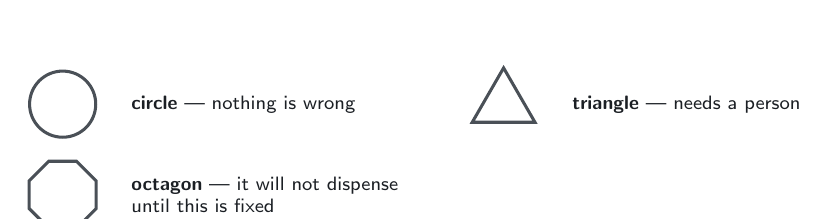
\begin{tikzpicture}[every node/.style={font=\sffamily\scriptsize, text=ink}]
  \draw[ink70, line width=1.1pt] (0,0) circle (0.42);
  \node[anchor=west] at (0.75,0) {\textbf{circle} \textemdash{} nothing is wrong};

  \begin{scope}[shift={(5.6,0)}]
    \draw[ink70, line width=1.1pt] (90:0.46) -- (210:0.46) -- (330:0.46) -- cycle;
    \node[anchor=west] at (0.75,0) {\textbf{triangle} \textemdash{} needs a person};
  \end{scope}

  \begin{scope}[shift={(0,-1.15)}]
    \draw[ink70, line width=1.1pt]
      (22.5:0.46) -- (67.5:0.46) -- (112.5:0.46) -- (157.5:0.46) --
      (202.5:0.46) -- (247.5:0.46) -- (292.5:0.46) -- (337.5:0.46) -- cycle;
    \node[anchor=west, align=left] at (0.75,0)
         {\textbf{octagon} \textemdash{} it will not dispense\\until this is fixed};
  \end{scope}
\end{tikzpicture}
\end{center}

\vspace{1mm}
\noindent The octagon is rare on purpose. A warning somebody sees three times a
day is a warning they stop reading.

\vspace{2mm}
\noindent\textbf{\sffamily The frame is three bands, and they never move.} A
status bar across the top carries seven fixed slots \textemdash{} wifi, relay,
clock, tray, power, coin cell, SD card \textemdash{} each an icon with a solid
severity shape under it, plus the wall clock. It never reorders and never
reflows, because a row you cannot learn is a row you have to read. An empty
field draws a dim icon and \emph{no} mark: absence is not a fault and is
certainly not a tick.

The middle band is the one dose that matters, with the time as the largest thing
on the panel and the tray number under the shape. Below it, a strip carries the
whole day: one solid mark per dose with its time under it, and a white divider
showing where you are. Taken is a blue circle, waiting a green circle, missed an
amber triangle, still to come a steel square \textemdash{} so ``did I take the
eight o'clock one'' is answered by looking.

The device's IP address sits permanently under the time. That matters more than
it sounds: Chrome on Android cannot resolve \code{pilldispenser.local}, so those
four numbers are the only way in for about half of everybody who tries \textemdash{}
and the screen that used to show them was part of a rotation that dropped it
exactly when there was an address to show.

\vspace{2mm}
\noindent\textbf{\sffamily A tap anywhere releases a dose.} There are no
on-screen buttons and nothing to aim at, deliberately: a target can be missed,
and this is a machine for hands that shake. Touching it also brings the panel
out of its night colours for half a minute.

\begin{provebox}
\provetitle
If the glass is dark, walk it one stage at a time:
\begin{shell}
sudo snapcare-dispenser --display-test
\end{shell}
It lights the backlight, floods red then green then blue, draws a windowed
rectangle and finally a real frame, asking after each what you can actually see
\textemdash{} then says what the first failure means. \code{--display-hz 8000000}
retries on a slower bus, which is the first thing to try on a speckled panel.

Then \code{selftest}. It paints each state in turn and asks which one you are
looking at, \textbf{what shape is on it}, and what colour. Those questions are
the whole test; answer them honestly.
\end{provebox}

\vspace{1mm}
\begin{dangerbox}
\dangertitle{A lit screen is not proof, and one wrong bit swaps two doses}
The LCD is write-only. A dead panel, an unplugged one and one wired a row off
all accept exactly the same writes without complaint, and the backlight comes on
regardless of whether anything is being drawn.

\vspace{1ex}
If the panel's BGR bit is wrong, red and blue trade places \textemdash{} so
\emph{released} and \emph{missed} swap, and the machine tells somebody their
pills are in the cup an hour after the window closed. That is why the self-test
asks what colour you can see and not whether you can see anything.
\end{dangerbox}

\clearpage

% ═══════════════════════════════════════════════════════════════════════════
\section{Stage 4 \textemdash{} the take-dose button (optional)}

The screen is already the control: a tap anywhere on the glass releases a
waiting dose, and Stage~3 fitted it. This stage adds a \emph{second}, physical
control, and it is worth two wires in exactly two situations \textemdash{} a
person who cannot reliably work a touch screen, and a bench where you want to
prove the release path without a finger on the glass.

Skip it otherwise. Both inputs reach the same \code{release()}, so nothing about
the machine's behaviour changes either way.

\vspace{3mm}
\begin{center}
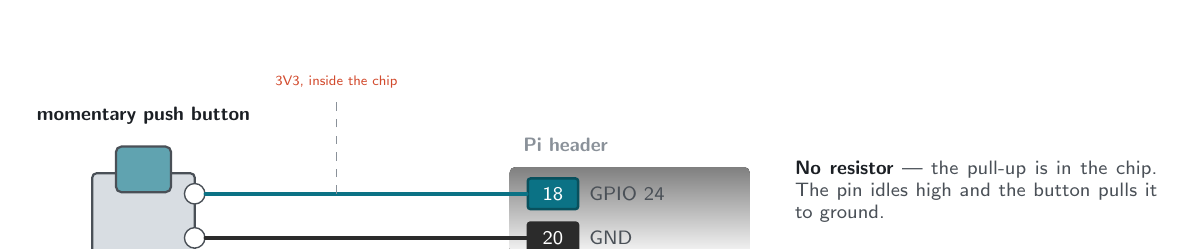
\begin{tikzpicture}
  \draw[ink70, line width=0.8pt, fill=ink15, rounded corners=1.5pt]
       (-4.3,-0.72) rectangle (-3.0,0.32);
  \draw[ink70, line width=0.8pt, fill=btnc!65, rounded corners=2pt]
       (-4.0,0.08) rectangle (-3.3,0.66);
  \node[font=\sffamily\scriptsize\bfseries, text=ink, anchor=south] at (-3.65,0.82)
       {momentary push button};

  \node[term] (ba) at (-3.0,0.06) {};
  \node[term] (bb) at (-3.0,-0.5) {};

  \hframe{1.55}{0.06}{-0.5}{Pi header}
  \hpin{1.55}{0.06}{18}{pusebtn}{GPIO 24}
  \hpin{1.55}{-0.5}{20}{pusegnd}{GND}

  \draw[wire, btnc] (ba) -- (H18.west);
  \draw[wire, gndc] (bb) -- (H20.west);

  \draw[ink40, line width=0.5pt, dashed] (-1.2,0.06) -- (-1.2,1.22);
  \node[font=\sffamily\tiny, text=p33, anchor=south] at (-1.2,1.28)
       {3V3, inside the chip};

  \node[font=\sffamily\scriptsize, text=ink70, align=left, anchor=north west]
       at (4.5,0.6)
       {\begin{minipage}{46mm}\scriptsize
        \textbf{\color{ink}No resistor} \textemdash{} the pull-up is in the chip.
        The pin idles high and the button pulls it to ground.\end{minipage}};
\end{tikzpicture}
\end{center}

\begin{dangerbox}
\dangertitle{It releases a due dose. It does not dispense}
Pressed when a dose is due, the tray sweeps. Pressed at any other time,
\textbf{nothing happens} \textemdash{} no tray moves and nothing is logged.

\vspace{1ex}
That is what stops a hopper being walked empty one press at a time by somebody
curious. Every one of those pills would be missing from a dose later in the
week, with nothing anywhere saying so.
\end{dangerbox}

\begin{provebox}
\provetitle
\code{selftest} asks you to press it once and reports what it counted.

\vspace{1.5ex}
\begin{tabular}{@{}>{\bfseries}l l@{}}
1 press seen   & pass \\
nothing seen   & open circuit \textemdash{} check the wire from pin 18 to pin 20 \\
4 presses seen & the debounce filter is not running \\
\end{tabular}

\vspace{1.5ex}
Then start the service and press it with no dose due:
\begin{shell}
journalctl -u snapcare-dispenser -f
\end{shell}
It must log \code{button pressed with no dose waiting} and open nothing. If a
tray moves here, stop and fix it.
\end{provebox}

\vspace{1mm}
\noindent A build with no button is the normal build: the screen and the app
both release doses without it.

\clearpage

% ═══════════════════════════════════════════════════════════════════════════
\section{Stage 5 \textemdash{} the servo rail, before any servo}

Wire the second supply and measure it with \textbf{no servos attached and no
signal wires to the Pi}. This is where a 12\,V brick or a reversed lead is
caught, while there is nothing connected for it to destroy.

\begin{provebox}
\provetitle
Meter across the rail with nothing attached: \textbf{5\,V $\pm$0.25\,V, steady}.
\end{provebox}

% ═══════════════════════════════════════════════════════════════════════════
\section{Stage 6 \textemdash{} the servos}

\vspace{2mm}
\begin{center}
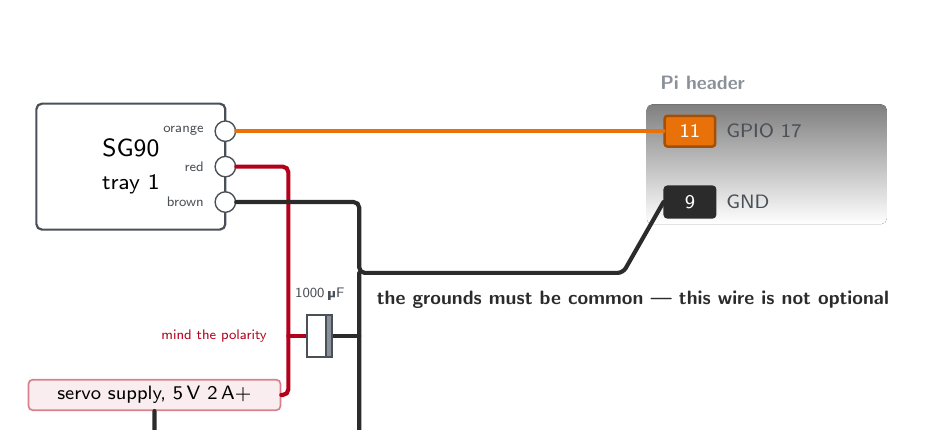
\begin{tikzpicture}
  \node[modbox, minimum width=24mm, minimum height=16mm] (sv) at (-4.4,0.0)
       {SG90\\[0.2ex]\footnotesize tray 1};
  \foreach \i/\name/\yy in {0/{orange}/0.45, 1/{red}/0.0, 2/{brown}/-0.45}{
    \node[term] (s\i) at (-3.2,\yy) {};
    \node[font=\sffamily\tiny, text=ink70, anchor=east] at (-3.35,\yy) {\name};
  }

  \hframe{2.7}{0.45}{-0.45}{Pi header}
  \hpin{2.7}{0.45}{11}{puseservo}{GPIO 17}
  \hpin{2.7}{-0.45}{9}{pusegnd}{GND}

  \node[compbox, minimum width=32mm, fill=p5!7, draw=p5!50] (rail) at (-4.1,-2.9)
       {servo supply, 5\,V 2\,A$+$};

  % the two rails
  \draw[wire, servo] (s0) -- (H11.west);
  \draw[wire, p5]    (s1) -- (-2.4,0.0) -- (-2.4,-2.9) -- (rail.east);
  \draw[wire, gndc]  (s2) -- (-1.5,-0.45) -- (-1.5,-1.35) -- (1.85,-1.35) -- (H9.west);
  \draw[wire, gndc]  (-1.5,-1.35) -- (-1.5,-3.45) -- (-4.1,-3.45) -- (rail.south);

  % the bulk capacitor, across the two rails and close to the servo
  \draw[wire, p5]   (-2.4,-2.15) -- (-2.16,-2.15);
  \draw[wire, gndc] (-1.84,-2.15) -- (-1.5,-2.15);
  \draw[ink70, line width=0.7pt, fill=white] (-2.16,-2.42) rectangle (-1.84,-1.88);
  \draw[ink70, line width=0.7pt, fill=ink40] (-1.92,-2.42) rectangle (-1.84,-1.88);
  \node[font=\sffamily\tiny, text=ink70, anchor=south] at (-2.0,-1.82) {1000\uF};
  \node[font=\sffamily\tiny, text=dangerred, anchor=east] at (-2.55,-2.15)
       {mind the polarity};

  \node[font=\sffamily\scriptsize\bfseries, text=gndc, anchor=north west] at (-1.4,-1.45)
       {the grounds must be common \textemdash{} this wire is not optional};
\end{tikzpicture}
\end{center}

\vspace{1mm}
\noindent Servos that twitch or ignore commands entirely read as a firmware
fault and are not one. It is this wire.

\vspace{3mm}
\noindent The other trays follow the same pattern, one signal wire each:

\begin{center}
\small
\begin{tabular}{@{}l c c c c c c c c@{}}
\toprule
\hdr{Tray} & 1 & 2 & 3 & 4 & 5 & 6 & 7 & 8 \\
\midrule
GPIO & 17 & 27 & 22 & 5 & 6 & 13 & 19 & 26 \\
Pin  & 11 & 13 & 15 & 29 & 31 & 33 & 35 & 37 \\
\bottomrule
\end{tabular}
\end{center}

\begin{provebox}
\provetitle
\textbf{One tray at a time}, and watch which hopper moves:
\begin{shell}
sudo snapcare-dispenser --drop 1     # then 2, then 3, six seconds apart
\end{shell}
\end{provebox}

\begin{dangerbox}
\dangertitle{``A tray moved'' is the wrong question}
Two trays wired to each other's pins both move, so a check that asks whether
something happened passes. The machine then gives the right number of pills from
the wrong compartment, and nobody notices until the wrong medication has been
taken for a week. Ask \emph{which one moved}.
\end{dangerbox}

\vspace{2mm}
\noindent\textbf{\sffamily Fit the horns with the servo parked.} Run
\code{-{}-drop} once and let it finish; the horn is then at rest. Nothing on an
SG90 reports its position, so a horn fitted while the servo happens to be at the
far end is a tray that never opens \textemdash{} and the dose is logged as
delivered anyway.

\vspace{2mm}
\noindent\textbf{\sffamily A servo buzzing at the end of its stroke} is being
driven past a stop it has already reached, and that one burns out over weeks.
Trim that tray alone, in microseconds:

\begin{shell}
# snapcare_dispenser/config.py
SERVO_TRIM = {3: (520, 2450)}
\end{shell}

\vspace{1mm}
\begin{warnbox}
\warntitle{All eight trays are accepted whether or not they exist}
An SG90 reports nothing, so the firmware cannot tell a missing hopper from a
fitted one. A schedule naming a tray you never built is accepted, never
dispensed, and reported by nothing. Say how many you have:
\begin{shell}
sudo systemctl edit snapcare-dispenser    # add: Environment=SNAPCARE_TRAYS=3
sudo systemctl restart snapcare-dispenser
\end{shell}
\end{warnbox}

% ═══════════════════════════════════════════════════════════════════════════
\section{Stage 7 \textemdash{} WiFi, by scanning a code}

Unplug the Ethernet cable. From here the machine joins a network the way its
owner will do it: by scanning a printed code. No keyboard, no monitor.

\begin{shell}
sudo snapcare-dispenser --show-qr     # the permanent setup network
sudo snapcare-dispenser --show-label  # everything the printed label must carry
\end{shell}

\begin{enumerate}[leftmargin=*, itemsep=0.5ex]
\item Print the code. It is derived from this board and \textbf{never changes},
      so it is printed once for the life of the device.
\item Scan it with a phone. The phone joins the dispenser's own network.
\item A setup page opens by itself. Pick the house network and type its password.
\item The dispenser joins it, its own network disappears, and the phone goes
      back to the house WiFi.
\end{enumerate}

\begin{provebox}
\provetitle
From the phone, on the house WiFi:
\code{http://pilldispenser.local/api/status} answers.

\vspace{1ex}
If that name does not resolve \textemdash{} Chrome on Android does no mDNS
\textemdash{} use the IP address the setup page showed you.
\end{provebox}

\vspace{1mm}
\begin{dangerbox}
\dangertitle{The pairing code on the label is a credential}
Anyone who can read it can send this device a schedule \emph{and release a
dose}. Put the label where the owner will find it and a visitor will not: inside
a battery door, or on the underside.
\end{dangerbox}

\vspace{1mm}
\noindent The QR carries your relay's address alongside the code, so reprint it
if you ever move relays. The code itself comes from the board and never changes.

\clearpage

% ═══════════════════════════════════════════════════════════════════════════
\section{Commissioning \textemdash{} six tests a bench cannot run}

\code{selftest} checks everything a program can check. These six it cannot, and
every one of them is a failure that looks exactly like a healthy machine.

\vspace{3mm}
\begin{center}
\small
\begin{tabular}{@{}>{\raggedright}p{32mm} >{\raggedright\arraybackslash}p{108mm}@{}}
\toprule
\hdr{Test} & \hdr{What to do, and what must happen} \\
\midrule
\textbf{The power cut} &
Pull the power at 08:30, after the 08:00 dose has been released, and restore it.
No second dose, and the log survives. Without persisted state this dispenses
twice, and no demo ever shows it \\
\textbf{The coin cell} &
Unplug the Pi, leave it a minute, bring it back with the network unplugged. The
clock must still be trusted and \code{clock.source} must read \code{rtc}. Nothing
on a bench with WiFi proves this, because NTP vouches first \\
\textbf{The wrong password} &
Type the WiFi password wrong on purpose at Stage~7. The setup network must come
back within seconds and say the password was refused. On a machine joined by
scanning a code, this is the difference between a second try and re-imaging the
card \\
\textbf{The internet cut} &
Pull the router's WAN cable, leave the phone and the dispenser on the LAN, and
release a due dose from the app. The pill must still come out. This catches a
release path that only works through the relay \\
\textbf{The dose nobody takes} &
Let a scheduled dose sit for its whole hour without pressing anything. The tray
must stay shut, the screen must go amber, and the log must record it missed. A
build that quietly drops it at the end has lost the point of asking first \\
\textbf{The idle button} &
Press the button with nothing due. Nothing must move and nothing must be
logged \\
\bottomrule
\end{tabular}
\end{center}

\vspace{4mm}
\noindent To make a dose fall due on demand, send a schedule for two minutes
from now:

\begin{shell}
curl "http://pilldispenser.local/schedule?payload=SC1*W*1:0800-127-000"
\end{shell}

\vspace{1mm}
\noindent\small
\code{SC1*W*}\emph{tray}\code{:}\emph{HHMM}\code{-}\emph{days}\code{-}\emph{length}.
Several times on one tray join with \code{.}, several trays with \code{/}.
\emph{days} is a bitmask with Monday as 1 \textemdash{} \code{127} is every day,
\code{021} is Mon/Wed/Fri. \emph{length} is a number of days, \code{000} for no
end date.
\normalsize

\clearpage

% ═══════════════════════════════════════════════════════════════════════════
\section{When it does not work}

\begin{center}
\small
\begin{longtable}{@{}>{\raggedright}p{50mm} >{\raggedright\arraybackslash}p{96mm}@{}}
\toprule
\hdr{Symptom} & \hdr{Look at} \\
\midrule
\endhead
\multicolumn{2}{@{}l}{\textbf{\sffamily Doses}}\\
The screen goes green and chirps, but no tray ever opens &
Working as designed. Something has to ask: the button, or release in the app \\
Pressing the button does nothing &
\code{gpio.button.presses} in \code{status}. Going up means the button works and
no dose was due. Staying at zero means the wire from pin 18 to pin 20 \\
Nothing is dispensed at all &
\code{device.blockedReason}. It is one of two things and they need opposite
fixes: an untrusted clock, or no GPIO library \\
Doses expire untaken every day &
Nobody is being told. Check \code{gpio.missing} for the buzzer \\
A tray in the schedule never dispenses &
It was accepted but never fitted. Set \code{SNAPCARE\_TRAYS} \\
\midrule
\multicolumn{2}{@{}l}{\textbf{\sffamily Screen}}\\
Nothing on the screen, ever &
\code{gpio.display} in \code{status}. \code{fitted:false} carries the reason \\
Lit, but nothing is ever drawn &
Very likely logic levels. A 5\,V module with a plain 74HC245 shifter needs
\textasciitilde3.5\,V to read a high and the Pi puts out 3.3\,V, so every line
reads low. Power VCC from 3V3 instead: a 3.3\,V board works, a 5\,V one goes
dark, and that tells you which you have \\
Backlight dark, not the picture &
LED is on a GPIO nobody drives. Set \code{SNAPCARE\_DISPLAY\_BACKLIGHT} to its
BCM pin; until then it sits low \\
A tap on the screen does nothing &
\code{sudo snapcare-dispenser -{}-touch-setup}. It says which of the four things
this is, and fixes the two it can \\
The log says it is ignoring an \code{ads7846} device &
A \code{dtoverlay=ads7846} line is still in \code{config.txt}. The firmware
refuses it rather than reading a panel that is not there; take the line out and
reboot \\
LCD: lit but blank &
The backlight is independent of the data lines, so a lit panel proves only that
LED has power. Check LCD\_RS (pin 22) and LCD\_RST (pin 12) \\
LCD: the colours are wrong &
The BGR bit. \emph{Released} and \emph{missed} swap when it is wrong; do not
ship it like this \\
LCD: mirrored or rotated &
\code{DISPLAY\_ROTATION} in \code{config.py} \\
\midrule
\multicolumn{2}{@{}l}{\textbf{\sffamily Servos and the clock}}\\
Servo twitches or ignores commands & The common ground. It is not optional \\
Servo hums between doses &
\code{gpio.servo.timing} \textemdash{} \code{python} is the slow fallback;
\code{sudo apt install python3-lgpio} \\
Pi reboots when a servo moves & Servos on the Pi's 5\,V pin, or no bulk capacitor \\
Clock right at shutdown, wrong at boot &
The cell is dead or not seated. \code{clock.rtc.detail} says which \\
\code{clock.rtc} says ``no record of ever having been set'' &
The chip has never been written. Set the clock once, then pull the power to
check it stuck \\
The RTC never changes after a \code{shutdown} and a boot &
A shutdown leaves the board powered, so nothing was tested. Pull the plug \\
\midrule
\multicolumn{2}{@{}l}{\textbf{\sffamily Network and install}}\\
\code{pilldispenser.local} does not resolve & Android does no mDNS. Use the IP address \\
Setup page never leaves ``waiting\ldots'' &
The phone has not gone back to the house WiFi. Switch it over \\
Setup page says no address was handed out &
The password was right and DHCP was not. Usually a router that needs restarting \\
A schedule request answers 421 &
The \code{Host} header is not a name this device answers to. Use
\code{pilldispenser.local} or the IP \\
\code{install.sh} stops on a dpkg lock &
Something else is mid-update. Wait, run it again, and do not delete the lock file \\
\bottomrule
\end{longtable}
\end{center}

% ═══════════════════════════════════════════════════════════════════════════
\section{Appendix \textemdash{} cloud sync, if you want it}

Without this the dispenser is LAN-only, which is a complete machine: the
schedule arrives over the house WiFi or off a photographed paper sheet, and the
SD card and the clock chip keep the alarms running.

With it, a schedule edited in the app reaches the device from anywhere, and a
carer in another country can release a dose. Deploy one relay for all your
devices \textemdash{} see \code{../cloud\_relay/} \textemdash{} then:

\begin{shell}
sudo systemctl edit snapcare-dispenser
# add: Environment=SNAPCARE_RELAY_URL=https://your-relay.example
sudo systemctl restart snapcare-dispenser
\end{shell}

\begin{provebox}
\provetitle
Pair the app with the code on the label. Then pull the router's WAN cable and
release a due dose from a phone on the same LAN: the pill still comes out. The
relay is a way in, never a dependency.
\end{provebox}

\vfill
\begin{center}\footnotesize\color{ink40}\sffamily
Generated from \code{docs/assembly-guide.tex} by \code{make guide}.\\
The pin map lives in \code{snapcare\_dispenser/config.py}, which is the source of truth.
\end{center}

\end{document}
